\setcounter{section}{1}
\setcounter{subsection}{6} % 1.7
\subsection{Router im Binärbaum}

Eine Gruppe von $2^n - 1$ Routern wird durch einen Binärbaum verbunden, wobei
sich an jedem Baumknoten ein Router befindet. Router $i$ kommuniziert mit
Router $j$ durch Senden einer Nachricht an die Wurzel des Baums. Die Wurzel
sendet die Nachricht nach $j$. Die Entfernung wird als Hop-Count gemessen,
d.h., jede durchlaufene Kante erhöht die Entfernung um 1.

\begin{enumerate}
    \item Zeichnen Sie den Binärbaum für $n = 3$ und erstellen Sie eine Tabelle
        mit allen Router-Paaren und deren Entfernung zu einander. Wie hoch ist
        die durchschnittliche Entfernung.

        \begin{minipage}{0.24\linewidth}
            \centering
            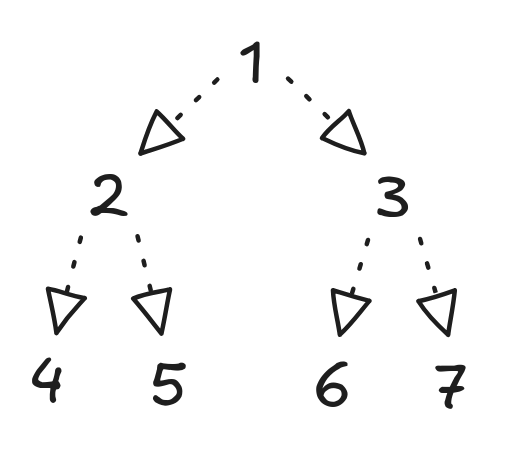
\includegraphics[width=1\textwidth]{./assets/1.7.a.png}
        \end{minipage}
        \begin{minipage}{0.24\linewidth}
            \centering
            \begin{tabular}{|c|c|}
                \hline
                Paar & Entf. \\
                \hline
                $(1, 2)$    & 1         \\
                \hline
                $(1, 3)$    & 1         \\
                \hline
                $(1, 4)$    & 2         \\
                \hline
                $(1, 5)$    & 2         \\
                \hline
                $(1, 6)$    & 2         \\
                \hline
                $(1, 7)$    & 2         \\
                \hline
                $(2, 3)$    & 2         \\
                \hline
            \end{tabular}
        \end{minipage}
        \begin{minipage}{0.24\linewidth}
            \centering
            \begin{tabular}{|c|c|}
                \hline
                Paar & Entf. \\
                \hline
                $(2, 4)$    & 3         \\
                \hline
                $(2, 5)$    & 3         \\
                \hline
                $(2, 6)$    & 3         \\
                \hline
                $(2, 7)$    & 3         \\
                \hline
                $(3, 4)$    & 3         \\
                \hline
                $(3, 5)$    & 3         \\
                \hline
                $(3, 6)$    & 3         \\
                \hline
            \end{tabular}
        \end{minipage}
        \begin{minipage}{0.24\linewidth}
            \centering
            \begin{tabular}{|c|c|}
                \hline
                Paar & Entf. \\
                \hline
                $(3, 7)$    & 3         \\
                \hline
                $(4, 5)$    & 4         \\
                \hline
                $(4, 6)$    & 4         \\
                \hline
                $(4, 7)$    & 4         \\
                \hline
                $(5, 6)$    & 4         \\
                \hline
                $(5, 7)$    & 4         \\
                \hline
                $(6, 7)$    & 4         \\
                \hline
            \end{tabular}
        \end{minipage}

        \begin{equation*}
            \overline{\text{Entfernung}} = \dfrac{60}{21} = 2.857142857
        \end{equation*}

    \item Verallgemeinern Sie die Überlegungen für beliebige große $n$. Leiten
        Sie eine Näherung für die durchschnittliche Anzahl der Teilstrecken pro
        Nachricht bei hohem $n$ ab unter der Annahme, dass alle Router-Paare
        gleichermaßen wahrscheinlich sind.

        Diese Lösung geht davon aus, dass es sich bei dem betrachteten
        Binärbaum um einen perfekten Binärbaum handelt – das heißt, jeder
        innere Knoten hat genau zwei Kindknoten und alle Blattknoten befinden
        sich auf derselben Ebene.

        Dann ist $2^n - 1$ die Gesamtanzahl der Knoten und $2^{k - 1}$ ist die
        Anzahl der Knoten in der Tiefe $k$.

        Sei $\text{L}_n := \{ ... \}$ die Menge aller Knoten in einem perfekten
        Bin"arbaum der Tiefe $n$, $\text{L}_{k,n} := \{ l \in \text{L}_n :
        \text{Tiefe}(l) = k \}$ die Menge der Knoten in der Tiefe $k$ und
        $S_n := \{(l_1, l_2) \in \text{L}_n^2\}$ die Menge aller Teilstrecken.

        Dazu definieren wir eine Abbildung $\text{d} : \{1,...,n\} \times
        \{1,...,n\} \rightarrow \mathbb{N}_0$, die die Entfernung aus einer
        Tiefe $k_1$ von einer anderen Tiefe $k_2$ zur"uckliefert.
        \begin{equation*}
            \text{d}(k_1, k_2) = (k_1 - 1) + (k_2 - 1)
        \end{equation*}
        Diese Formel basiert auf der Bedingung, dass Nachrichten immer über die
        Wurzel des Baums geroutet werden.

        Die durchschnittliche Anzahl der Teilstrecken pro Nachricht wird durch
        die Funktion $\overline{\text{d}} : \mathbb{N}_{+}
        \rightarrow \mathbb{N}_{0}$ berechnet, definiert als
        \begin{equation*}
            \overline{\text{d}}(n) = \dfrac{\sum_{i = 1}^n \sum_{j = 1}^n |L_{i,n}
                \times L_{j,n}| \cdot \text{d}(i, j)}{|S_n|}
        \end{equation*}
        wobei gilt:
        \begin{itemize}
            \item $\text{d(i, j)}$ ist die Entfernung zwischen einem Knoten auf
                Tiefe $i$ und einem Knoten auf Tiefe $j$,
            \item $L_{i,n}$ (bzw. $L_{j,n}$) bezeichnet die Menge der Knoten auf Tiefe $i$ (bzw. $j$),
            \item $|L_{i,n} \times L_{j,n}|$ ist die Anzahl aller m"oglichen Paare von
                Knoten auf den Tiefen $i$ und $j$,
            \item $|S_n|$ ist die Gesamtanzahl aller m"oglichen Knotenpaare in
                einem Bin"arbaum der Tiefe $n$.
        \end{itemize}
        Dies lässt sich durch eine Reihe algebraischer Umformungen wie folgt
        vereinfachen (die Herleitung wurde zur Übersichtlichkeit weggelassen):
        \begin{equation*}
            \overline{\text{d}}(n) = \dfrac{2^{2n + 1}n - 2^{2n + 2} - 2^{n + 1}n + 2^{n + 3} - 4}{(2^n - 1)^2}
        \end{equation*}
\end{enumerate}
